\section{Study 2: Awareness with Impact}
\label{study:impact}

In response to Study 1, a second investigation was conducted. Study 1 revealed
that pairs of developers can be used around technical dependencies in order
to predict bugs. The natural follow up to these findings was to conduct a study
of indirect conflicts surrounding these developer pairs that are involved in 
source code changes. These indirect
conflicts were primarily studies through the notion of task awareness.

%Awareness tools
Tools have been created to attempt to solve task awareness related issues
with some success~\cite{Xiang:2008:ERT, Biehl:2007:FVD, Sarma:2009:TIV, Khurana:2009:PFC}. 
These tools have been designed 
to solve task awareness related issues at the direct conflict level. 
Examples of direct conflict awareness include knowing when two or more 
developers are  editing same artifact, finding expert knowledge of a
particular file, and knowing which developers are working on which files.
On the other hand, task awareness related issues at the indirect conflict level
have also been studied, with many tools being
produced~\cite{Sarma:2007:TSA,Servant:2010:CPI,Begel:2010:CDE,Trainer:2005:BGT}. 
Examples of indirect conflict awareness
include having one's own code effected by another developer's source
code change or finding out who might be indirectly effected by one's
own code change. Previous interviews and surveys conducted with software developers have 
shown a pattern that developers of a software project view indirect conflict 
awareness  as a high priority issue in their development~\cite{Damian:2007:GSE, 
Halverson:2006:DTV, Begel:2010:CDE, Schroter:2012:TTF}.

% Limitations of indirect conflict tools
Indirect conflicts arising in source code are inherently
difficult to resolve as most of the time, source code analysis or
program slicing~\cite{Weiser:1982:PUS} must
be performed in order to find relationships between technical objects
which are harmed by changes.
While some awareness tools have been created with these indirect conflicts
primarily in mind~\cite{Begel:2010:CDE, Trainer:2005:BGT}, most have only 
created an exploratory environment which is used by developers to
solve conflicts which may arise~\cite{Servant:2010:CPI}. These tools were not designed to detect
indirect conflicts that arise and alert developers to their presence 
inside the software system. Sarma et al.~\cite{Sarma:2007:TSA} has started to work directly
on solving indirect conflicts, however, these products are not designed to handle
internal structures of technical objects.

%Outline of study
In this study, I report on research into supporting developer pairs in indirect conflicts
and present the design, and implementation of the tool \textit{Impact},
a web based tool that aims at detecting indirect conflicts among developers
and notifying the appropriate members involved in these conflicts. Through Impact and
its evaluation I ask:

\begin{description}
        \item[RQ\namedlabel{itm:rq1-impact}{RQ1-Impact}] \textit{Can indirect conflicts be supported 
        through an awareness mechanism which leverages pairs of developers whose changing technical 
        dependencies statistically relate to bugs?}
\end{description}

By leveraging technical relationships inherent of 
software projects with method call graphs~\cite{Lakhotia:1993:CCM}
as well as detecting changes
to these technical relationship through software configuration management
(SCM) systems, \textit{Impact} is able to detect indirect conflicts as well as
alert developers involved in such conflicts in task awareness while limiting information
overload by using design by contract~\cite{Meyer:1988} solutions to method design. While this study
outlines \textit{Impact's} specific implementation, its design is rather
generic and can be implemented in similar indirect conflict awareness tools.

After a brief evaluation of \textit{Impact} with two student software teams, it was
found that \textit{Impact} suffers from information overload and a high false positive rate which turn out to be quite
large problems found in many other indirect conflict
tools~\cite{Sarma:2007:TSA, Holmes:2010:CAR, Trainer:2005:BGT, Servant:2010:CPI, Borici:2012:CHA}.

\subsection{Related Work}
Although there is an abundance of awareness tools developed in research
today, only a handful have made an attempt to examine indirect conflicts.
Here, I will outline four of the forefront projects in indirect conflicts
and how these projects have influenced the decision making process in
the design and implementation of \textit{Impact}.

I first start with both Codebook~\cite{Begel:2010:CDE} and 
Ariadne~\cite{Trainer:2005:BGT}. These projects produce an exploratory
environment for developers to handle indirect conflicts. Exploratory
pertains to the ability to solve self determined conflicts, meaning that
once a developer discovers a conflict, they can use the tool as a type of
lookup table to solve their issue. Codebook is a type of social developer
network that relates developers to source code, issue repositories and
other social media while Ariadne only examines their source code for developer
to source code association. Through Codebook, developers become
owners of source code artifacts. Both projects also use program 
dependency graphs~\cite{Horwitz:1992:UPD}
in order to relate technical artifacts to each other. These projects make 
use of method call graphs in order to 
determine which methods invoke others which forms the basis for 
linking source code artifacts creating a directed graph. While these 
projects can be great tools 
for solving indirect conflicts which may arise, by querying such directed
graphs to view impacts of conflict creating code, they lack the ability to
detect potential conflicts on their own.

A serious attempt at both detecting and informing developers of
indirect conflicts is the tool Palantir~\cite{Sarma:2007:TSA}. Palantir
monitors developer's activities in files with regards to class signatures.
Once a developer changes the signature of a class, such as by modifying changes
in name, parameters, or return values of public methods, any workspace
of other developers which are using that class will be notified. Palantir utilizes
a push-based event model~\cite{Fitzpatrick:2002:SPA} which seems to be
a favored collection system among awareness tools. Sarma et al.
~\cite{Sarma:2007:TSA} also
developed a generic design for future indirect conflict awareness tools. 
However, Palantir falls short in its collection and distribution
mechanisms. First, Palantir only considers ``outside'' appearance of technical
objects, being their return types, parameters, etc. Secondly, Palantir 
only delivers
detected conflicts to developers who are presently viewing or editing
the indirect object while other developers who have used the modified 
class previously are not notified.

I will lastly examine the tool CASI~\cite{Servant:2010:CPI} which uses
a sphere of influence for each developer to determine how source code
changes are indirectly related to other components of the software.
CASI uses dependency slicing~\cite{Bajracharya:2009:SIS} instead of the 
call graphs in Ariadne~\cite{Trainer:2005:BGT} which gives dependencies among
all source code entities. This provides a verbose output of dependencies when
source code is changed. CASI also implements a visualization where
a developer can see what parts of a software projects he or she may be effecting
with the source code change. This allows the developers themselves to go and fix
potential issues elsewhere in the project before the code change is committed
to the software repository. While CASI covers great ground in its approach,
it still leaves the issue of information overload, although attempts were made
to solve this by having severity levels of indirect conflicts presented to
the user.

\subsection{Impact}
This section will proceed to give an outlined detail of \textit{Impact} in both its
design and implementation. The design of \textit{Impact} was created to be
a generic construct which can be applied to other indirect conflict 
awareness tools while the implementation is specific to the technical
goals of \textit{Impact}.

\subsubsection{Design}
Compared to tool design for direct conflicts, the major concern of 
indirect conflict tools is to relate technical objects to one another
with a ``uses'' relationship. To say that object 1 uses object 2 is to infer
a technical relationship between the two objects which can be used
in part to detect indirect conflict that arise from modifying object
2. This kind of relationship is modeled based on directed graphs ~\cite{Horwitz:1992:UPD}. 
Each technical object is represented by node while each ``uses''
relationship is represented by a directed edge. This representation
is used to indicate all indirect relationships within a software project.

\begin{figure}[t!]
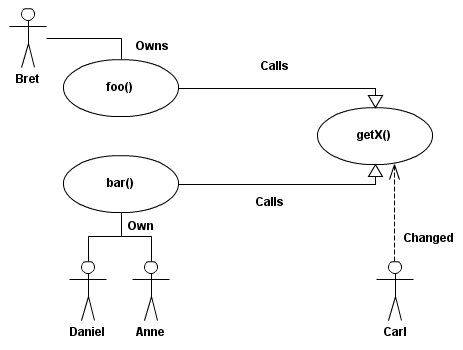
\includegraphics[width=\columnwidth]{figures/CallGraph}
\caption{Technical object directed graph with ownership\label{fig:graph}}
\end{figure}

While technical object relationships form the basis of indirect conflicts,
communication between developers is my ultimate goal of resolving such conflicts
(as was seen in Study 1).
This being the case, developer ownership must be placed on the 
identified technical objects. With this ownership, I now infer
relationships among developers based on their technical objects
``uses'' relationship. Developer A, who owns object 1, which uses 
object 2 owned by developer B, may be notified by a change to
object 2's internal workings. Most, if not all, ownership information
of technical objects can be extracted from a project's source code
repository (CVS, Git, SVN, etc.).

Finally, the indirect conflict tool must be able to detect changes
to the technical objects defined above and notify the appropriate owners
to the conflict. 
Two approaches have been 
proposed for change gathering techniques: real time and commit 
time~\cite{Fitzpatrick:2002:SPA}.
I propose the use of commit time
information gathering as it avoids the issue of developers 
overwriting previous work or deleting modifications which would 
produce information for changes that no longer exist. However, the
trade off is that indirect conflicts must be committed before detected,
which results in conflicts being integrated into the system before being able
to be dealt with as opposed to catching conflicts before they happen.
At commit time, the tool must parse changed source code in relation
to technical artifacts in the created directed graph detailed above.
Where \textit{Impact's} design differs from that of Palantir's is that
the object's entire body (method definition and internal body) is 
parsed, similar to that of CASI~\cite{Servant:2010:CPI},
at commit time, as opposed to real time, to detect changes anywhere in the technical object.
This is a first design step towards avoiding information overload.
Once technical objects are found to be changed, appropriate owners
of objects which use the changed object should be notified. 
In Figure~\ref{fig:graph}, Carl changes method (technical object) 1,
which effects methods 2 and 3 resulting in the alerting of
developers Bret, Daniel, and Anne. I have opted to alert the invoking
developers rather than the developer making the change to potential
solutions as my conflicts are detected at commit time and this supports
the idea of a socio-technical congruence~\cite{Kwan:2011:ESC} 
from software structure to communication patterns in awareness systems.

With this three step design: (i) creating directed graphs of technical
objects, (ii) assigning ownership to those technical objects, and (iii)
detecting changes at commit time and the dissemination of conflict information
to appropriate owners, I believe a wide variety of
indirect conflict awareness tools can be created or extended.

\subsubsection{Implementation}
For \textit{Impact's} implementation, I decided to focus on methods as my
selected technical objects to infer a directed graph from. The ``uses'' 
relationship described above for methods is method invocation.
Thus, in my constructed dependency graph, methods represent nodes
and method invocations represent the directed edges. In order to 
construct this directed graph, abstract syntax trees (ASTs) are 
constructed from source files in the project.

Once the directed graph is constructed, I must now assign
ownership to the technical objects (methods) as per the design.
To do this, I simply query the source code repository. In this case
I used Git as the source code repository, so the command \textit{git blame}
is used for querying ownership information. (Most source code 
repositories have similar commands and functionality.) This command 
returns the source code authors per line which can be used to assign
ownership to methods.

To detect changes to technical objects (methods), I simply 
use a commit's \textit{diff} which is a representation of all changes
made inside a commit. I can use the lines changed in the \textit{diff} to 
find methods that have been changed. This gives cause of potential
indirect conflicts. 
I now find all methods in the directed graphs which invoke these changed methods. 
These are the final indirect conflicts.

Once the indirect conflicts have been found, I use the
ownership information of technical objects to send notifications to
those developers involved in the indirect conflict. All owners
of methods which invoke those that have been changed are alerted
to the newly changed method. Impact can been seen in
Figure~\ref{fig:impact}, the user interface of \textit{Impact}. Here, in an RSS type
feed, the changing developer, time of change, changed method,
invoking methods, and commit message are all displayed. 
The weight provided is the percent changed of changed method multiplied by 
ownership of the invoking method. This allows developers to filter
through high and low changes affecting their own source code.

\begin{figure}[t!]
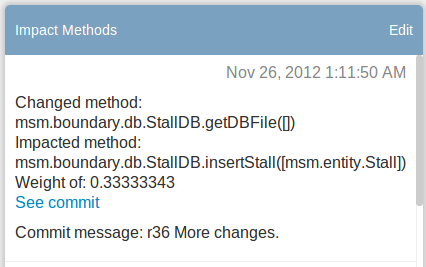
\includegraphics[width=\columnwidth]{figures/ImpactDemo}
\caption{\textit{Impact's} RSS type information feed.\label{fig:impact}}
\end{figure}

\subsection{Evaluation}
To fully evaluate both the generic design of detecting and resolving
indirect conflicts as well as \textit{Impact}, extensive testing and evaluation
must be performed. However, I felt that a simple evaluation is
first needed to assess the foundation of \textit{Impact}'s design and claims
about indirect conflicts at the method level.

I performed a user case study where I gave \textit{Impact} to 
two small development teams composed of three developers. Each team was
free to use \textit{Impact} at their leisure during their development process,
after which interviews were conducted with lead developers from 
each development team. The interviews were conducted after each
team had used \textit{Impact} for three weeks.

I asked lead developers to address two main concerns: do indirect
conflicts pose a threat
at the method level (e.g. method 1 has a bug because it invokes method
2 which has had its implementation changed recently), 
and did \textit{Impact} help raise
awareness and promote quicker conflict resolution for indirect
conflicts. The two interviews largely supported the expectation of
indirect conflicts posing a serious threat to developers, especially
in medium to large teams or projects as opposed to the small
teams which they were a part of. It was also pointed
out that method use can be a particularly large area for indirect
conflicts to arise. However, it was noted that
any technical object which is used as an interface to some data
construct or methodology, database access for instance, can be 
a large potential issue for indirect conflicts.  Interview responses to
\textit{Impact} were optimistically positive, as interviewees stated that \textit{Impact}
had potential to raise awareness among their teams with what other developers
are doing as well as the influence it has on their own work. However,
\textit{Impact} was shown to have a major problem of information overload. 
It was suggested
that while all method changes were being detected,
not all are notification worthy. One developer suggested to only notify
developers if the internal structure of a method
changes due to modification to input parameters or output parameters.
In other words, the boundaries of the technical objects (changing
how a parameter is used inside the method, modifying the return
result inside the method) seem to be more of interest than other 
internal workings. More complex inner workings of methods were also noted 
to be of interest to developers
such as cyclomatic complexity, or time and space requirements.

These two studies have shown that my design and approach to
detecting and alerting developers to indirect conflicts appear
to be on the correct path. However, \textit{Impact} has clearly shown
the Achilles heel of indirect conflict tools, which is information
overload because of an inability to detect ``notification worthy''
changes.

\subsection{Threats to Validity}
Because of the tool validation nature of this work, I chose participant interviews as my research validation method, which has some implications regarding the
limitations and threats to validity of this study. While I did have some positive results regarding the potential of Impact in this study,
populations studied from outside of this study's participants may add new insights into the pool of findings. As a result of this, findings
from this study may not relate to everyone or generalize to outside of the group of participants involved in this study.

I conducted this case study with undergraduate students at the University of Victoria. This being said, participants
may not have had enough real world experience to validate this study at an industry level. The students were also consumed with their regular course
work which could have limited the time spent using Impact and the enthusiasm put forward while conducting this study.

To counter this, my study was conducted purely on a volunteer basis to eliminate those participants which may have been to busy to focus
on the study or provide appropriate feedback where needed.

\subsection{Conclusions of Study}
\label{sec:ns}
In this study, I have proposed a generic 
design for the development of awareness tools in regards to
handling indirect conflicts. I have presented a prototype 
awareness tool, \textit{Impact}, which was designed around the generic 
technical object approach. However, \textit{Impact} suffered from
information overload, in that it had too many notifications sent to
developers.

A potential solution to information overload comes from the ideas of
Meyer~\cite{Meyer:1988} on ``design by contract''. In this methodology, changes to method
preconditions and postconditions are considered to be the most harmful. 
This includes adding conditions that must be met by both input
and output parameters such as limitations to input and expected
output. To achieve this level of source code analysis, the ideas of
Fluri et al.~\cite{Fluri:2007:CDT} can be used on the previously generated
ASTs for high granularity
source code change extraction when determining if preconditions or
postconditions have changed.

Aside from better static analysis tools for examining source code changes,
the results of this study potentially imply a lack of understanding into the
root causes of indirect conflicts.  A theme of information overload to developers
continues to crop up in indirect conflicts, of which the root cause should
be examined in future studies.